\begin{minipage}{.2\textwidth}
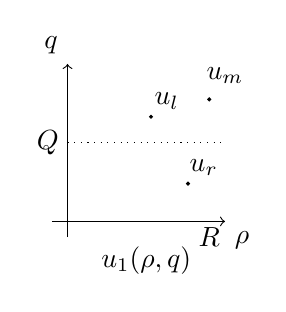
\begin{tikzpicture}
% coordinates
\draw[->] (0,-0.2) -- (0,2) node[anchor= south east] {$q$};
\draw[->] (-0.2,0) -- (2,0) node[anchor= north west] {$\rho$};
% rarefactions
%\draw[cyan!50] (1, 1.3) -- (2, 1.6) ;
%\draw[<-][lime] (0, 1) -- (1, 1.3) ;
%\draw[->][cyan!50] (0, 1) -- (2, 0.4) ;


\draw[lime, domain=0:2]  plot[id=x] function{0.31*x +1};
\draw[black!30, domain=0:2]  plot[id=x] function{-0.34*x +1};
\draw[dotted] (0,1) -- (2, 1);
% contact disk
\draw[black!30, domain=0:1.28]  plot[id=x] function{(x/1.16)*(2-1.16)/(2-x)*1.63};
\draw[orange!50, domain=0:1.86]  plot[id=x] function{(x/1.38)*(2-1.38)/(2-x)*0.33};
% initial conditions
\node at (1.06+0.2, 1.33+0.2) {$u_l$};
\node at (1.53+0.2, 0.48+0.2) {$u_r$};
\node at (1.8+0.2, 1.55+0.3) {$u_m$};
\filldraw[black] (1.06, 1.33) circle (0.5pt);  % u_1
\filldraw[black] (1.53, 0.48) circle (0.5pt);   % u_2
\filldraw[black] (1.8, 1.55) circle (0.5pt);   % u_m
%labels
\node at (1.8, -0.2) {$R$};
\node at (-0.25, 1) {$Q$};
\node at (1, -0.5) {$u_1(\rho, q)$};
\end{tikzpicture}
\end{minipage}
\begin{minipage}{.2\textwidth}
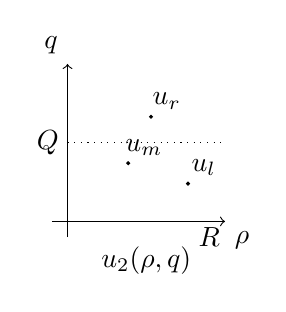
\begin{tikzpicture}
% coordinates
\draw[->] (0,-0.2) -- (0,2) node[anchor= south east] {$q$};
\draw[->] (-0.2,0) -- (2,0) node[anchor= north west] {$\rho$};
% rarefactions
%\draw[cyan!50] (1, 1.3) -- (2, 1.6) ;
%\draw[<-][lime] (0, 1) -- (1, 1.3) ;
%\draw[->][cyan!50] (0, 1) -- (2, 0.4) ;
\draw[black!30, domain=0:2]  plot[id=x] function{0.31*x +1};
\draw[lime, domain=0:2]  plot[id=x] function{-0.34*x +1};
\draw[dotted] (0,1) -- (2, 1);
% contact disk
\draw[orange!50, domain=0:1.28]  plot[id=x] function{(x/1.16)*(2-1.16)/(2-x)*1.63};
\draw[black!30, domain=0:1.86]  plot[id=x] function{(x/1.38)*(2-1.38)/(2-x)*0.33};
% initial conditions
\node at (1.06+0.2, 1.33+0.2) {$u_r$};
\node at (1.53+0.2, 0.48+0.2) {$u_l$};
\node at (0.77+0.2, 0.74+0.2) {$u_m$};
\filldraw[black] (0.77, 0.74) circle (0.5pt);   % u_m
\filldraw[black] (1.06, 1.33) circle (0.5pt);  % u_1
\filldraw[black] (1.53, 0.48) circle (0.5pt);   % u_2
%labels
\node at (1.8, -0.2) {$R$};
\node at (-0.25, 1) {$Q$};
\node at (1, -0.5) {$u_2(\rho,q)$};
\end{tikzpicture}
\end{minipage}
\quad
\begin{minipage}{.2\textwidth}
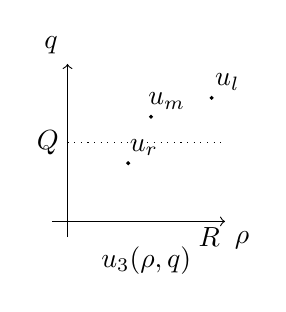
\begin{tikzpicture}
% coordinates
\draw[->] (0,-0.2) -- (0,2) node[anchor= south east] {$q$};
\draw[->] (-0.2,0) -- (2,0) node[anchor= north west] {$\rho$};
% rarefactions
%\draw[cyan!50] (1, 1.3) -- (2, 1.6) ;
%\draw[<-][lime] (0, 1) -- (1, 1.3) ;
%\draw[->][cyan!50] (0, 1) -- (2, 0.4) ;
\draw[cyan!50, domain=0:2]  plot[id=x] function{0.31*x +1};
\draw[black!30, domain=0:2]  plot[id=x] function{-0.34*x +1};
\draw[dotted] (0,1) -- (2, 1);
% contact disk
\draw[orange!50, domain=0:1.28]  plot[id=x] function{(x/1.16)*(2-1.16)/(2-x)*1.63};
\draw[black!30, domain=0:1.86]  plot[id=x] function{(x/1.38)*(2-1.38)/(2-x)*0.33};
% initial conditions
\node at (1.83+0.2, 1.57+0.2) {$u_l$};
\node at (0.77+0.2, 0.74+0.2) {$u_r$};
\node at (1.06+0.2, 1.33+0.2) {$u_m$};
\filldraw[black] (1.83, 1.57) circle (0.5pt);  % u_1
\filldraw[black] (0.77, 0.74) circle (0.5pt);   % u_2
\filldraw[black] (1.06, 1.33) circle (0.5pt);  % u_m
%labels
\node at (1.8, -0.2) {$R$};
\node at (-0.25, 1) {$Q$};
\node at (1, -0.5) {$u_3(\rho,q)$};
\end{tikzpicture}
\end{minipage}
\begin{minipage}{.2\textwidth}
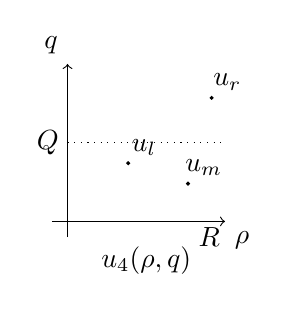
\begin{tikzpicture}
% coordinates
\draw[->] (0,-0.2) -- (0,2) node[anchor= south east] {$q$};
\draw[->] (-0.2,0) -- (2,0) node[anchor= north west] {$\rho$};
% rarefactions
%\draw[cyan!50] (1, 1.3) -- (2, 1.6) ;
%\draw[<-][lime] (0, 1) -- (1, 1.3) ;
%\draw[->][cyan!50] (0, 1) -- (2, 0.4) ;
\draw[black!30, domain=0:2]  plot[id=x] function{0.31*x +1};
\draw[cyan!50, domain=0:2]  plot[id=x] function{-0.34*x +1};
\draw[dotted] (0,1) -- (2, 1);
% contact disk
\draw[black!30, domain=0:1.28]  plot[id=x] function{(x/1.16)*(2-1.16)/(2-x)*1.63};
\draw[orange!50, domain=0:1.86]  plot[id=x] function{(x/1.38)*(2-1.38)/(2-x)*0.33};
% initial conditions
\node at (1.83+0.2, 1.57+0.2) {$u_r$};
\node at (0.77+0.2, 0.74+0.2) {$u_l$};
\node at (1.53+0.2, 0.48+0.2) {$u_m$};
\filldraw[black] (1.83, 1.57) circle (0.5pt);  % u_1
\filldraw[black] (0.77, 0.74) circle (0.5pt);   % u_2
\filldraw[black] (1.53, 0.48) circle (0.5pt);  % u_m
%labels
\node at (1.8, -0.2) {$R$};
\node at (-0.25, 1) {$Q$};
\node at (1, -0.5) {$u_4(\rho, q)$};
\end{tikzpicture}
\end{minipage}